\documentclass{mldsmsc}
% \setlength{\parindent}{20pt}

\title{Probabilistic Matrix Factorisation Algorithms for 12-lead ECG Data}
\author{Joana Levtcheva}
\CID{01252821}
\supervisor{Dr Deniz Akyildiz}
% \date{1 May 2023}
%For today's date, use:
\date{\today}
\logoimg{}


% THIS IS WHERE NEW COMMANDS CAN BE DEFINED
% commands below only used in the proof; otherwise can be deleted
\newcommand{\consta}{a}
\newcommand{\X}{X}
\newcommand{\EE}[1]{ \mathrm{E} [ #1 ] }
\newcommand{\inparenth}[1]{\left( #1 \right)}

\begin{document}

% Generates the Title Page
\maketitle


% Generates plagiarism declaration
\declarationname{Joana Levtcheva}
\declarationdate{\today}
\declaration 


\begin{abstract}
Probabilistic matrix factorisation for high-deimensional time-series data with nonlinear subspace: 12-lead ECG data exploration \newline

\noindent Example: In recent years, matrix factorisation (MF) algorithms have gained popularity in the field of machine learning and have found applications in various fields, such as recommendation systems, image processing and missing data imputation. The MF problem concerns factorising a high dimensional data matrix into two lower dimensional factors. The aim of MF methods is to find the factors such that we have a lower dimensional representation of the data.\newline

\noindent In this thesis, we propose a novel

\begin{acknowledgements}

I would like to...

\end{acknowledgements}

% add glossary?

% table of contents
\tableofcontents

% VERY IMPORTANT
% This command switches from Roman to Arabic numbering for main part of thesis
\mainmatter


\chapter{Introduction}

Matrix factorisation (MF) techniques are highly effective and widely used in unsupervised machine learning. Simply said (LA context), the methods decompose the original matrix into multiple lower-dimensional? matrices. By breaking the matrix in these simpler components MF aim to uncover latent structures that are not immediately apparent in the original matrix. Some applications are in image processing: for reducing dimensionality and noise in images, NLP for topic modelling, word embeddings, etc... \newline

\noindent Introduce mathrmatical nottation here as well:

\begin{equation}
Y \approx CX
\end{equation}

\begin{equation}
\underbrace{
\begin{bmatrix}
  \times & \times & \times & \times \\
  \times & \times & \times & \times \\
  \times & \times & \times & \times
\end{bmatrix}
}_{\text{Y $\in \mathbb{R}^{m \times n}$ }}
\approx
\underbrace{
\begin{bmatrix}
  \times & \times \\
  \times & \times \\
  \times & \times
\end{bmatrix}
}_{\text{C $\in \mathbb{R}^{m \times r}$ }}
\underbrace{
\begin{bmatrix}
  \times & \times & \times & \times \\
  \times & \times & \times & \times
\end{bmatrix}
}_{\text{X $\in \mathbb{R}^{r \times n}$ }}
\end{equation}

\noindent There are also probabilistic versions of MF which incorporate probabilistic models to better handle uncertainty and variability in the data. They not only decompose the matrix but also provide probabilistic interpretations of the factors. Despite considerable progression in the probabilistic versions, there is demand for such methods in applications such as uncertainty quantification, managing time-series data, and executing efficient probabilistic components. \newline

\hline

Matrix factorisation (Linear algebra case -> factorisation into multiple...) computational/numerical LA and so on... \\

MF in the ML context ... \\

Our context and problem... \\

The introduction section goes here\footnote{Tip: write this section last.}.
Matrix factorisation (MF) algorithms... \\

\hline

\noindent The paper "Probabilistic matrix factorisation" (PMF) (\cite{NIPS2007_d7322ed7}) introduces an efficient and scalable model for collaborative filtering. The algorithm performs well on large, sparse and im- balanced datasets. This is demonstrated by using a Netflix dataset, alongside with an adaptive prior to control model complexity, and a constrained version to handle users with few ratings. PMF treats each rating as an independent event which means that the time varying component is not taken into consideration, and the algorithm is not suitable for sequential data. \newline

\noindent In the paper "Dictionary Filtering: A Probabilistic Approach to Online Matrix Factorization" (\cite{cite-key}), the authors introduce a novel online MF algorithm known as dictionary filtering. It leverages probabilistic models, specifically using recursive linear filters, and efficiently factorises the original data matrix into a dictionary matrix and a coefficients matrix. This is an online algorithm, meaning it is suitable for high-dimensional and time-varying data, and it also has easy to tune parameters. Although the model can learn nonstationary and dynamic data, it is developed for linear and Gaussian state space models (SSM). (Particularly for ECG data, ECG has a nonlinear SSM which doesn't suit the dictionary filtering.) -> Efficient for high-dimensional data, adaptable to non-stationary environments, removes the need for step-size tuning; flexible and computationally efficient: $O(mr^2)$ independent of the number of data points. \newline

\noindent Later, Akyildiz et.al. develop Probabilistic Sequential Matrix Factorization (PSMF) (\cite{akyildiz2021probabilistic}). This method is tailored to time-varying and non-stationary datasets consisting of high-dimensional time-series. Nonlinear Gaussian SSM are considered, decomposing the original matrix into a dictionary matrix and time-variying coefficient matrix. This time, the matrices are with potentially nonlinear dependencies. The model is demonstrated to work on tasks such as forecasting, changepoint detection, missing data imputation, and is shown to work on real-world data with a periodic subspace. There is also a robust version using Student-t filters to handle model misspecification. -> PSMF efficiently captures temporal dependencies through Markovian structures on the coefficients, making it possible to encode the dependencies into a lower dimensional latent space. Strengths: Handles non-stationary and time-varying data, robust to model misspecification, efficient sequen- tial inference. Suitable for: modelling data with periodic subpaces, high-dimensional data by reducing it to lower-dimensional latent space, data imputation,
Weaknesses: Potential problems with very large datasets, having many data points. \newline

\noindent In the unpublished MSc thesis (Imperial College London) of Rina Maletta (\cite{rina}), the author introduces Matrix-Variate Gaussian Matrix Factorization (MVGMF). This is a novel PMF method using matrix-variate Gaussian distributions. The algorithm has fast Gaussian updates which take the form of a preconditioned MF algorithm which is stable. An extension for handling missing data and data imputation is also proposed. The method is tested on the Netflix Prize dataset, London air quality (NO2) data, and Olivetti face image dataset.

\section{Contributions}

PSMF applied to 12-lead ECG data -> imputation, forecasting, R peaks detection \\

Multiple Fourier terms, higher rank for this case (check the paper) \\

Why R peaks is important \\

Not many algoorithms, processing, ... espiecially not Probabilistic \\

\section{Notation}

Mathematics notation $f_{\theta}$

\section{ECG/medical introduction}

PQRST complex, R-peak..., diagram, data

\chapter{Background}

Background chapter.

\section{Prelims}

Section content goes here. 

\subsection{PMF}

A subsection.

\subsection{DF}

Section content goes here.

\subsection{PSMF}

Section content goes here.

\subsection{NMF}

Section content goes here.

\subsection{MVGMF}

Section content goes here.

\section{Figures}

It is better to create figures in a vector-based format, such as PDF.

\begin{figure}[!h]
    \centering
    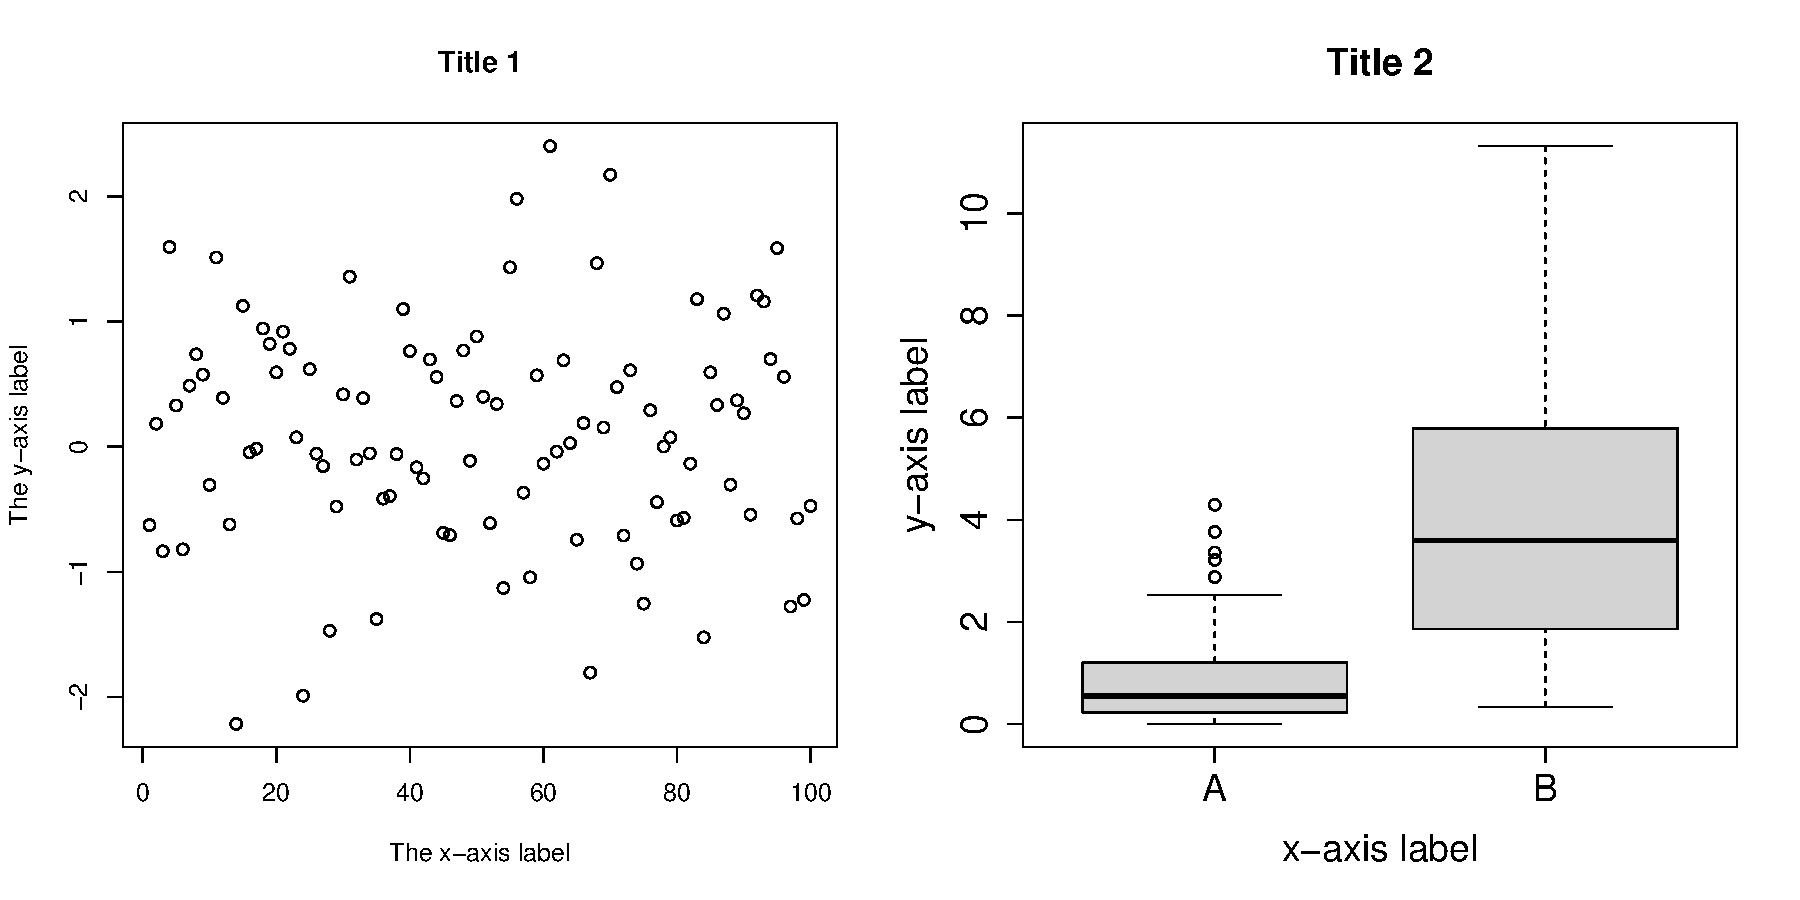
\includegraphics[width=\textwidth]{fig1.pdf}
    \caption{Remember to make fonts in figures large enough (compare the two figures.)}
    \label{fig:fig1}
\end{figure}

\section{Tables}

\label{sec:tablesection}

Here is an example of a table

\begin{table}[ht]
\centering
\begin{tabular}{rr}
  \hline
    $z$& $\textrm{P}(Z < z)$ \\
  \hline
    1.281& 0.900\\
    1.645& 0.950\\
    1.960& 0.975\\
    2.326& 0.990 \\
    2.576& 0.995 \\
   \hline
\end{tabular}
    \caption{Partial table showing values of $z$ for $\textrm{P}(Z < z)$, 
    where $Z$ has a standard normal distribution.}
    \label{tab:normal}
\end{table}



\section{Referencing sources, sections and items}

A good book on the bootstrap is \cite{cite1}, although the idea
appeared in an earlier paper \citep{cite1}.

Note that to make the references appear, you will need to compile
the bibtex, otherwise you may just see question marks where the references
should be.


\subsection{Referencing sections, results and equations}

Theorem~\ref{thm:theorem1} is proved in Section~\ref{sec:defnthms}; see 
Equation~\eqref{eqn:second}.



\subsubsection{Referencing tables and figures}

When labelling figures and tables, it is important that the label command
\texttt{\textbackslash label\{LABELNAME\}} comes \textbf{after} the caption command.
See Table~\ref{tab:normal} and Figure~\ref{fig:fig1} above.

\subsection{Quoting sources}
If you wish to quote a source, be sure to use quotation marks and cite the
reference. The \texttt{\textbackslash{usequote}} command is useful here:

\usequote{It was the best of times, it was the worst of times, it was the age of wisdom, it was the age of foolishness, it was the epoch of belief, it was the epoch of incredulity, it was the season of Light, it was the season of Darkness, it was the spring of hope, it was the winter of despair, we had everything before us, we had nothing before us, we were all going direct to Heaven, we were all going direct the other way - in short, the period was so far like the present period, that some of its noisiest authorities insisted on its being received, for good or for evil, in the superlative degree of comparison only.} \citep{cite1}

% forcing a page break
\clearpage


\section{Definitions, theorems and examples}
\label{sec:defnthms}

The following environments are supported:
Definition, Theorem, Proof, Proposition, Lemma, Remark, Example.

\begin{definition}
    The \textbf{variance} of a random variable $X$ is defined as
    \begin{equation}
        \mathrm{Var}(X) = \mathrm{E}[(X - \mathrm{E}[X])^2].
    \end{equation}
\end{definition}

\begin{theorem}
    \label{thm:theorem1}
Given a random variable $X$, over all values $a \in \mathbb{R}$, 
\begin{equation}
    \min_{a \in \mathbb{R}} \mathrm{E}[(X - a)^2] 
    = \mathrm{E}[(X - \mathrm{E}[X])^2].
    \label{eqn:second}
\end{equation}
\end{theorem}

\begin{proof}   
    Starting with the left-hand side,
\begin{align}
% Example of using \newcommands; see above
\EE{ \inparenth{\X - \consta}^2 } 
&=  \EE{  \inparenth{\X - \EE{\X} + \EE{\X} - \consta}^2 } 
    \nonumber \\
&=  \EE{  \inparenth{ \X - \EE{\X} }^2 } 
    + 2 \EE{ \inparenth{ \X - \EE{\X} } \inparenth{ \EE{\X} - \consta} } +  
  \EE{ \inparenth{ \EE{\X} - \consta}^2  }    
    \nonumber \\
&=  \EE{  \inparenth{ \X - \EE{\X} }^2 } +  \inparenth{ \EE{\X} - \consta}^2
    \nonumber \\
& \geq \EE{  \inparenth{ \X - \EE{\X} }^2 },  
\nonumber 
\end{align}
since $\EE{\X}$ is a real number and $\inparenth{ \EE{\X} - \consta}^2 \geq 0$,
and the third line follows from linearity of expectation:
\begin{align}
    \EE{ \inparenth{ \X - \EE{\X} } \inparenth{ \EE{\X} - \consta} }
    =
    \inparenth{ \EE{\X} - \consta} \EE{ \inparenth{ \X - \EE{\X} } }
    =
    \inparenth{ \EE{\X} - \consta}  \inparenth{\EE{ \X} - \EE{\X} } 
    =
    0,
    \nonumber
\end{align}
    since $\EE{\EE{\X}} = \EE{\X}$, which proves the result.
\end{proof}

\begin{remark}
    This theorem shows that that the minimum of the quantity
    $\mathrm{E}[(X - a)^2]$ is equal to $\mathrm{Var}(X)$.
    In some sense, this makes the variance a natural measure of dispersion if 
    we are taking the metric to be the squared deviation of $X$.
\end{remark}


\begin{lemma}[Stein's Lemma]
    Let $X \sim \mathrm{N}(\mu, \sigma^2)$, and let $g$ be a differentiable 
    function satisfying $\mathrm{E}[|g'(X)|] < \infty$. Then
    \begin{equation}
        \mathrm{E}[g(X)(X-\mu)] = \sigma^2 \mathrm{E}[g'(X)].
        \nonumber
    \end{equation}
\end{lemma}

\begin{proposition}[Popoviciu's inequality]
    Suppose that the random variable $X$ is known to only take values in the 
    bounded range $[a, b]$. Then  
    \begin{align}
        \mathrm{Var}[X] \leq \dfrac{(b-a)^2}{4}.
        \nonumber
    \end{align}
\end{proposition}

\begin{example}
    Suppose $X \sim \mathrm{Bern} (p)$, for some $p \in [0,1]$. Then, 
    since $X \in \{0, 1\}$, $X$ is bounded between $0$ and $1$ and so
    $\mathrm{Var}[X] \leq \tfrac{1}{4}$.
\end{example}

\chapter{PSMF/etc for ECG}

Describe algorithm \\

Focus on the application to ECG data -> challenges, characteristics, data pre, post, processing 

\chapter{Experiemnts and Results}

Some text

Pre,post, processing

What exactly is tested -> 5k points, sample from the points, results, smoothing, no smoothing, differrnt ranks, fourier terms

\section{Missing data}

Both algorithms

\section{R peaks?}

Original - Forecast -> for R peaks detection

One paper about NMF

Scipy function

remove the reconstruction from the original signal

\section{Forecasting}

This fails 

- issues, R-peak

Lower frequency is better -> rank 6, fourier terms 6, iterations 100, 200, 500, leraning rate

%% DO NOT EDIT - AUTOMATICALLY GENERATED FROM RESULTS!
%% This table requires booktabs and multirow!
%% Table for missing percentage 20
\begin{tabular}{lc}
\toprule
 & ECG \\
\cmidrule(lr){2-2}
PSMF & 0.39 \\
rPSMF & \textbf{0.85} \\
MLE-SMF & 0.18 \\
\bottomrule
\end{tabular}

%% DO NOT EDIT - AUTOMATICALLY GENERATED FROM RESULTS!
%% This table requires booktabs and multirow!
%% Table for missing percentage 30
\begin{tabular}{lc}
\toprule
 & ECG \\
\cmidrule(lr){2-2}
PSMF & 0.32 \\
rPSMF & \textbf{0.79} \\
MLE-SMF & 0.17 \\
\bottomrule
\end{tabular}

%% DO NOT EDIT - AUTOMATICALLY GENERATED FROM RESULTS!
%% This table requires booktabs and multirow!
%% Table for missing percentage 40
\begin{tabular}{lc}
\toprule
 & ECG \\
\cmidrule(lr){2-2}
PSMF & 0.24 \\
rPSMF & \textbf{0.70} \\
MLE-SMF & 0.15 \\
\bottomrule
\end{tabular}

%% DO NOT EDIT - AUTOMATICALLY GENERATED FROM RESULTS!
%% This table requires booktabs, amsmath, and multirow!
\begin{tabular}{lrr}
\toprule
 & \multicolumn{1}{c}{Imputation RMSE} & \multicolumn{1}{c}{Runtime (s)} \\\cmidrule(lr){2-6} \cmidrule(lr){7-11}
 & ECG & ECG \\ \cmidrule(lr){2-6} \cmidrule(lr){7-11}
PSMF & $\underset{{\scriptscriptstyle \;\;(18.06)}}{\textbf{62.79}}$ & 1.02\\
rPSMF & $\underset{{\scriptscriptstyle \;\;(17.57)}}{63.32}$ & 1.21\\
MLE-SMF & $\underset{{\scriptscriptstyle \;\;\;(21.13)}}{251.06}$ & 1.19\\
TMF & $\underset{{\scriptscriptstyle \;\;\;(15.05)}}{172.87}$ & 0.57\\
PMF* & $\underset{{\scriptscriptstyle \;\;\;(nan)}}{nan}$ & 0.21\\
\bottomrule
\end{tabular}

%% DO NOT EDIT - AUTOMATICALLY GENERATED FROM RESULTS!
%% This table requires booktabs, amsmath, and multirow!
\begin{tabular}{lrr}
\toprule
 & \multicolumn{1}{c}{Imputation RMSE} & \multicolumn{1}{c}{Runtime (s)} \\\cmidrule(lr){2-6} \cmidrule(lr){7-11}
 & ECG & ECG \\ \cmidrule(lr){2-6} \cmidrule(lr){7-11}
PSMF & $\underset{{\scriptscriptstyle \;\;(19.76)}}{78.93}$ & 1.07\\
rPSMF & $\underset{{\scriptscriptstyle \;\;(16.56)}}{\textbf{73.74}}$ & 1.11\\
MLE-SMF & $\underset{{\scriptscriptstyle \;\;\;(82.96)}}{267.00}$ & 0.93\\
TMF & $\underset{{\scriptscriptstyle \;\;\;(17.25)}}{166.36}$ & 0.43\\
PMF* & $\underset{{\scriptscriptstyle \;\;\;(nan)}}{nan}$ & 0.18\\
\bottomrule
\end{tabular}

%% DO NOT EDIT - AUTOMATICALLY GENERATED FROM RESULTS!
%% This table requires booktabs, amsmath, and multirow!
\begin{tabular}{lrr}
\toprule
 & \multicolumn{1}{c}{Imputation RMSE} & \multicolumn{1}{c}{Runtime (s)} \\\cmidrule(lr){2-6} \cmidrule(lr){7-11}
 & ECG & ECG \\ \cmidrule(lr){2-6} \cmidrule(lr){7-11}
PSMF & $\underset{{\scriptscriptstyle \;\;\;(21.92)}}{106.57}$ & 1.01\\
rPSMF & $\underset{{\scriptscriptstyle \;\;(22.32)}}{\textbf{96.08}}$ & 1.10\\
MLE-SMF & $\underset{{\scriptscriptstyle \;\;\;(61.04)}}{268.91}$ & 0.92\\
TMF & $\underset{{\scriptscriptstyle \;\;\;(20.59)}}{157.12}$ & 0.45\\
PMF* & $\underset{{\scriptscriptstyle \;\;\;(nan)}}{nan}$ & 0.16\\
\bottomrule
\end{tabular}

\chapter{Conclusion}

data imputation 

forecasting challneged or success

R-peaks

\section{Future work}

More complex model etc...

Faster computation, etc...

Conclusion goes here. 





\clearpage
 %% reset page counter and start appendix pages with A
\pagenumbering{arabic}
\renewcommand*{\thepage}{A\arabic{page}}

%% Appendix goes here
%\appendix
%
%\chapter{Appendix title}
%
%Appendix goes here.


%%References part of appendices
% References: modify the file refs.bib
\bibliographystyle{plainnat}
\bibliography{refs}


\end{document}
